%!TEX encoding = UTF-8 Unicode
%!TEX root = ../compendium2.tex

\Teamlab{\LabWeekTEN}

\begin{Goals}
%!TEX encoding = UTF-8 Unicode
%!TEX root = ../compendium2.tex

\item Kunna använda arv.
\item Kunna göra överskuggning av medlemmar i en supertyp.
%\item Kunna referera till medlemmar i superklassen med \code{super} vid överskuggning.
\item Kunna förklara begreppet dynamisk bindning.
\item Kunna använda abstrakta klasser och skapa en klasshierarki.

\end{Goals}

\begin{Preparations}
\item Gör övning {\tt \ExeWeekNINE} i kapitel \ref{exe:W09}, speciellt uppgift \ref{exe:inheritance:labprep-pair}.
\item Läs dokumentationen för \code{introprog.BlockGame}.
\item Läs igenom hela laborationen och förbered dig inför första gruppmötet.
%!TEX encoding = UTF-8 Unicode
%!TEX root = compendium.tex
\item 
Diskutera i din samarbetsgrupp hur ni ska dela upp koden mellan er i flera olika delar, som ni kan arbeta med var för sig. En sådan del kan vara en klass, en trait, ett objekt, ett paket, eller en funktion. 
\item
Varje del ska ha en \emph{huvudansvarig} individ. 
\item
Arbetsfördelningen ska vara någorlunda jämnt fördelad mellan gruppmedlemmarna.
\item
När ni redovisar er lösning ska ni börja med att redogöra för handledaren hur ni delat upp koden och vem som är huvudansvarig för vad. 
\item
Den som är huvudansvarig för en viss del redovisar den delen.
\item 
Grupplaborationer görs i huvudsak som hemuppgift. Salstiden används primärt för redovisning.
\item Träffas i din samarbetsgrupp och diskutera ert arbetssätt utifrån följande frågeställningar:
\begin{itemize}[nolistsep]
  \item Vilka krav ska ni implementera?
  \item Hur ska ni jobba med gemensamma koddelar?
  \item Hur ska ni dela med er av de koddelar som ni utvecklar var för sig?
\end{itemize}

\end{Preparations}

\subsection{Bakgrund}

Spelet \emph{Snake}\footnote{Även kallat ''masken''. \url{https://sv.wikipedia.org/wiki/Snake}} blev mäkta populärt i Sverige redan på 1980-talet, ofta spelat på den legendariska datorn ABC80. Spelet finns i flera varianter, både för en spelare och som duell mellan två spelare. Varje spelare styr en mask med huvud och svans som hela tiden rör sig framåt. Det gäller att undvika att köra in i en masksvans och att samla poäng t.ex. genom att äta äpple.

Figur~\ref{fig:snake-game} visar en startdialog där man kan välja antal spelare, samt ett exempel på spel med en och två spelare. I varianten för en spelare närmar sig maskens huvud äpplet och lyckas kanske äta det om spelaren styr rätt.  I varianten för två spelare vinner grön mask eftersom den blåa masken råkade köra in i den gröna maskens svans.
\begin{figure}[H]
\begin{minipage}{0.45\textwidth}
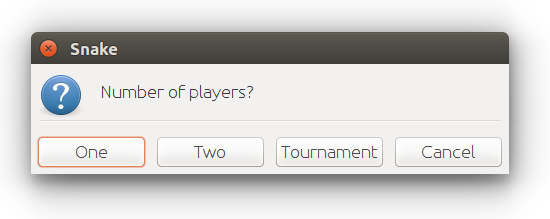
\includegraphics[width=1.0\textwidth]{../img/snake-start}

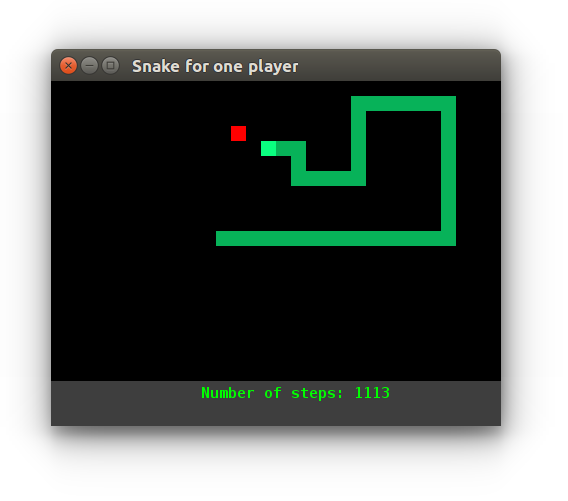
\includegraphics[width=1.0\textwidth]{../img/snake-oneplayer}
\end{minipage}
\begin{minipage}{0.5\textwidth}
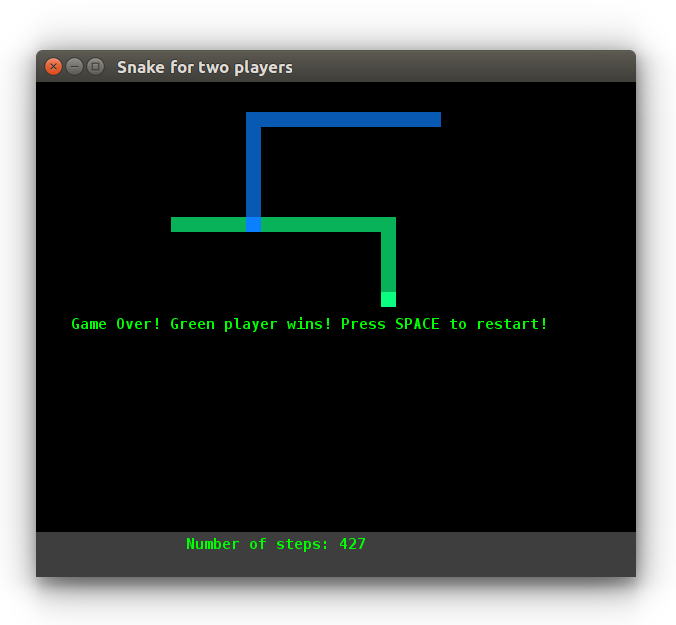
\includegraphics[width=1.0\textwidth]{../img/snake-twoplayer}
\end{minipage}
\caption{Spelet snake för en spelare med äpple och för två spelare utan äpple. \label{fig:snake-game}}
\end{figure}

\subsection{Obligatoriska funktionella krav}

Följande funktionella krav ska uppfyllas av ert program om ni är sex personer i gruppen. Om ni är färre ingår de obligatoriska krav som visas i tabell \ref{lab:snak:table-reqt}.
%\footnote{Om någon student, p.g.a. långvarig sjukdom eller annat giltigt skäl, genomför laborationen själv i efterhand som en individuell laboration ska följande krav implementeras på egen hand: \code{Player}, \code{OnePlayerGame}, \code{Snake}, \code{Apple}.}
\begin{itemize}[nosep, label={$\square$},]
\item \textbf{\texttt{Player}}. Det ska finnas spelare som motsvarar mänskliga användare och som har ett namn och fyra tangenter som den kan spela med. Varje spelare har en egen orm som den kan styra med sina tangenter.

\item \textbf{\texttt{Snake}}. Det ska finnas ormar. En orm består av ett antal block, där det främsta blocket kallas huvud och resten av blocken kallas svans. Huvudet har en ljusare färg än kroppen. Svansens längd ökar under spelets gång. En orm rör sig i en viss riktning och varje spelare kan ändra riktningen på sin orm med sina tangenter, i en av fyra riktningar \code{North}, \code{South}, \code{East} eller \code{West}.

\item \textbf{\texttt{Apple}}. Det ska finnas (minst ett) äpple. Ett äpple består av ett rött block och finns på en slumpvis position. Ett äpple kan ätas av en orm om ormens huvud träffar äpplet. Varje gång ett äpple äts upp av en orm så teleporteras äpplet till en ny position och kan ätas igen.

\item \textbf{\texttt{Banana}}. Det ska finnas (minst en) banan. En banan består av tre vertikala gula block och finns på en slumpvis position. En banan äts upp av en orm om ormens huvud träffar bananen. Varje gång en banan äts upp av en orm så teleporteras bananen till en ny slumpvis position och kan ätas igen.

\item \textbf{\texttt{Monster}}. Det ska finnas (minst ett) monster. Ett monster består av fem rosa block i kryssform.  Ett monster föds på en slumpvis position och rör sig i en riktning som bestäms vid monstrets födelse. Ett orm blir uppäten och dör om ormens huvud nuddar ett monsterblock .

\item \textbf{\texttt{OneplayerGame}}. Det ska gå att spela ensam. I varianten med en spelare finns en orm och minst ett äpple (och ev. även bananer och monster). Varje gång användarens orm lyckas äta en frukt får användaren poäng. När ormen ätit ett visst antal äpplen, eller om ormen blivit uppäten av ett monster, är spelet slut och poängen visas. En ormsvans ska bli längre vid jämna tidsintervall eller om den äter frukt.

\item \textbf{\texttt{TwoplayerGame}}. Det ska gå att spela två och två. I varianten med två spelare finns två ormar. Det finns också äpplen, bananer och monster. Om en orm äter en banan blir dess svans längre. När ormen ätit ett visst antal äpplen, eller om ormen blivit uppäten av ett monster, är spelet slut och poängen visas. En ormsvans ska bli längre vid jämna tidsintervall eller om den äter frukt.

\item \textbf{\texttt{Settings}}. Inställningar för spelet ska vara konfigurerbara genom en textfil som laddas i början av spelet. Inställningar ska vara en kontextparameter.  

\end{itemize}
\begin{table}[H]
  \centering
  \caption{Krav som minst ska implementeras vid respektive gruppstorlek. Om du har särskilda skäl kan du efter godkännande från kursansvarig göra labben enskilt.  \label{lab:snak:table-reqt}}

\begin{tabular}{r | c c c c c c}
  Krav / Antal personer & 1       & 2       & 3       & 4       & 5       & 6 \\ \hline
  \texttt{Player}       & $\surd$ & $\surd$ & $\surd$ & $\surd$ & $\surd$ & $\surd$ \\
  \texttt{OnePlayerGame}& $\surd$ &         &         &         & $\surd$ & $\surd$ \\
  \texttt{TwoPlayerGame}&         & $\surd$ & $\surd$ & $\surd$ & $\surd$ & $\surd$ \\
  \texttt{Snake}        & $\surd$ & $\surd$ & $\surd$ & $\surd$ & $\surd$ & $\surd$ \\
  \texttt{Apple}        & $\surd$ &         & $\surd$ & $\surd$ & $\surd$ & $\surd$ \\
  \texttt{Banana}       &         &         &         & $\surd$ &         & $\surd$ \\
  \texttt{Monster}      &         &         & $\surd$ &         &         & $\surd$ \\
  \texttt{Settings}     & $\surd$ & $\surd$ & $\surd$ & $\surd$ & $\surd$ & $\surd$ \\
\end{tabular}
\end{table}

\subsection{Obligatoriska design-krav}

\begin{enumerate}[label={$\square$}, leftmargin=*]

\item Snake-spel ska gå att starta med huvudprogrammet nedan. Huvudprogrammet får ändras vid behov i enlighet med minimikrav vad gäller gruppstorlek i tabell \ref{lab:snak:table-reqt}, samt valbara extrakrav i avsnitt \ref{lab:snake:extra-reqts}, och era egna ideer.
\scalainputlisting{../workspace/w10_snake/Main.scala}

\item Spelet ska bygga vidare på \code{introprog.BlockGame} enligt typhierarkin i fig.~\ref{snake:fig:game-hierarchy}.

\begin{figure}[H]
\begin{center}
\newcommand{\TextBox}[1]{\raisebox{0pt}[1em][0.5em]{#1}}
\tikzstyle{umlclass}=[rectangle, draw=black,  thick, anchor=north, text width=3cm, rectangle split, rectangle split parts = 3]
\begin{tikzpicture}[inner sep=0.5em,scale=1.0, every node/.style={transform shape}]

  \node [umlclass, rectangle split parts = 1, xshift=0cm, yshift=4.5cm] (BaseType)  {
              \textit{\textbf{\centerline{\TextBox{\code{BlockGame}}}}}
%              \nodepart[align=left]{second}\code{def x: T} \newline \code{def y: T}
          };


  \node [umlclass, rectangle split parts = 1, xshift=0cm, yshift=3.0cm] (SubType)  {
              \textit{\textbf{\centerline{\TextBox{\code{SnakeGame}}}}}
%              \nodepart[align=left]{second}\code{val x: Int} \newline \code{val y: Int}
          };

\node [umlclass, rectangle split parts = 1, xshift=-3cm, yshift=1.0cm] (SubSubType1)  {
            {\textbf{\centerline{\TextBox{\code{OnePlayerGame}}}}}
%            \nodepart[]{second}\TextBox{\code{val dim: Int}}
        };

\node [umlclass, rectangle split parts = 1, xshift=3cm, yshift=1.0cm] (SubSubType2)  {
            {\textbf{\centerline{\TextBox{\code{TwoPlayerGame}}}}}
%            \nodepart[]{second}\TextBox{\code{val dim: Int}}
        };

\draw[umlarrow] (SubType.north) -- ++(0,0.5) -| (BaseType.south);
\draw[umlarrow] (SubSubType1.north) -- ++(0,0.5) -| (SubType.south);
\draw[umlarrow] (SubSubType2.north) -- ++(0,0.5) -| (SubType.south);

\end{tikzpicture}
\end{center}
\caption{Arvshierarki med klassen \code{introprog.BlockGame} som bastyp.}
\label{snake:fig:game-hierarchy}
\end{figure}


\item Ormar, monster och frukt ska utgå från bastypen \code{Entity} enligt typhierarkin i ~\ref{snake:fig:entity-hierarchy}.

\begin{figure}[H]
\begin{center}
\newcommand{\TextBox}[1]{\raisebox{0pt}[1em][0.5em]{#1}}
\tikzstyle{umlclass}=[rectangle, draw=black,  thick, anchor=north, text width=2.5cm, rectangle split, rectangle split parts = 3]
\begin{tikzpicture}[inner sep=0.5em,scale=1.0, every node/.style={transform shape}]

  \node [umlclass, rectangle split parts = 1, xshift=0.0cm, yshift=4.5cm] (BaseType)  {
              \textit{\textbf{\centerline{\TextBox{\code{Entity}}}}}
%              \nodepart[align=left]{second}\code{def x: T} \newline \code{def y: T}
          };


  \node [umlclass, rectangle split parts = 1, xshift=-3.0cm, yshift=2.5cm] (SubType1)  {
              \textit{\textbf{\centerline{\TextBox{\code{CanMove}}}}}
%              \nodepart[align=left]{second}\code{val x: Int} \newline \code{val y: Int}
          };

\node [umlclass, rectangle split parts = 1, xshift=-4.75cm, yshift=0.5cm] (SubSubType01)  {
            {\textbf{\centerline{\TextBox{\code{Snake}}}}}
%            \nodepart[]{second}\TextBox{\code{val dim: Int}}
};

\node [umlclass, rectangle split parts = 1, xshift=-1.5cm, yshift=0.5cm] (SubSubType02)  {
            {\textbf{\centerline{\TextBox{\code{Monster}}}}}
%            \nodepart[]{second}\TextBox{\code{val dim: Int}}
};


\node [umlclass, rectangle split parts = 1, xshift=3.0cm, yshift=2.5cm] (SubType2)  {
            \textit{\textbf{\centerline{\TextBox{\code{CanTeleport}}}}}
%            \nodepart[]{second}\TextBox{\code{val dim: Int}}
        };

\node [umlclass, rectangle split parts = 1, xshift=1.75cm, yshift=0.5cm] (SubSubType1)  {
            {\textbf{\centerline{\TextBox{\code{Apple}}}}}
%            \nodepart[]{second}\TextBox{\code{val dim: Int}}
        };

\node [umlclass, rectangle split parts = 1, xshift=5.0cm, yshift=0.5cm] (SubSubType2)  {
            {\textbf{\centerline{\TextBox{\code{Banana}}}}}
%            \nodepart[]{second}\TextBox{\code{val dim: Int}}
        };


\draw[umlarrow] (SubType1.north) -- ++(0,0.5) -| (BaseType.south);
\draw[umlarrow] (SubType2.north) -- ++(0,0.5) -| (BaseType.south);
\draw[umlarrow] (SubSubType1.north) -- ++(0,0.5) -| (SubType2.south);
\draw[umlarrow] (SubSubType2.north) -- ++(0,0.5) -| (SubType2.south);
\draw[umlarrow] (SubSubType01.north) -- ++(0,0.5) -| (SubType1.south);
\draw[umlarrow] (SubSubType02.north) -- ++(0,0.5) -| (SubType1.south);

\end{tikzpicture}
\end{center}
\caption{Arvshierarki med klassen \code{Entity} som bastyp.}
\label{snake:fig:entity-hierarchy}
\end{figure}


\item \code{Entity} representerar en varelse i ett spel och ska se ut så här:
\scalainputlisting{../workspace/w10_snake/Entity.scala}
% \begin{Code}
% trait Entity {
%   def draw():   Unit
%   def erase():  Unit
%   def update(): Unit
%   def reset():  Unit
% }
% \end{Code}
Metoderna \code{draw} resp. \code{erase} anropas vid ritning resp. radering. Metoden \code{reset} återställer ursprungstillståndet. Metoden \code{update} anropas en gång i varje runda i spel-loopen. Predikatet \code{isOccupyingBlockAt} ger sant om positionen \code{p} finns bland de block som varelsen ockuperar på skärmen.

\item \code{CanMove} representerar en entitet som kan röra sig i en viss hastighet, enligt:
\scalainputlisting{../workspace/w10_snake/CanMove.scala}

% \begin{Code}
% trait MovingEntity extends Entity {
%   def move(): Unit
%
%   var movesPerSecond: Double = 20.0
%
%   final def millisBetweenMoves(): Int =
%     (1000 / movesPerSecond).round.toInt max 1
%
%   private var _timestampLastMove: Long = System.currentTimeMillis
%   final def timestampLastMove = _timestampLastMove
%
%   override final def update(): Unit =
%     if (System.currentTimeMillis > _
%           timestampLastMove + millisBetweenMoves) {
%       _timestampLastMove = System.currentTimeMillis
%       move()
%     }
% }
% \end{Code}

\item \code{CanTeleport} representerar en entitet som finns på en viss plats men som efter ett visst antal uppdateringar utan förvarning teleporterar sig till en ny position:
\scalainputlisting{../workspace/w10_snake/CanTeleport.scala}

\item Det ska finnas en enumeration \code{State} i singelobjektet \code{SnakeGame} som representerar spelets övergripande tillstånd enligt följande:
\begin{Code}
package snake 

object SnakeGame:
  enum State:
    case Starting, Playing, GameOver, Quitting
  export State.* // gör alla tillstånd synliga i SnakeGame
\end{Code}

\item Vid varje runda i spelloopen ska följande logik exekveras. Denna kod placeras förslagsvis i \code{gameLoopAction}, se vidare \code{SnakeGame} i avsnitt \ref{lab:snake:tips}.
\begin{Code}
    if state == Playing && !isPaused then
      _iterationsSinceStart += 1
      entities.foreach(_.erase())
      entities.foreach(_.update())
      entities.foreach(_.draw())
      onIteration()
      if isGameOver then enterGameOverState()
\end{Code}

\item Det ska finnas ett singelobjekt \code{Colors} där alla färger som används i spelet samlas.

\item Filen \code{pairs.scala} ska enligt laborationsförberedelser i övningsuppgift   \ref{exe:inheritance:labprep-pair} på sidan \pageref{exe:inheritance:labprep-pair} innehålla
\code{Pair[T]}, \code{Dim}, \code{Pos}, \code{Dir}, \code{North}, \code{South}, \code{East}, \code{West}. Se workspace här:\\
\url{https://github.com/lunduniversity/introprog/tree/master/workspace/}

\item Klassen \code{Player} ska se ut som följer:

\end{enumerate}

\scalainputlisting[basicstyle=\ttfamily\fontsize{10.5}{13}\selectfont]
{../workspace/w10_snake/Player.scala}




\subsection{Valbara krav -- varje person ska välja minst ett}\label{lab:snake:extra-reqts}

Varje person i gruppen ska implementera \emph{minst ett} (gärna flera) av kraven nedan. Vid implementation av flera av dessa krav blir spelet väsentligt roligare.
\begin{itemize}[nosep, label={$\square$}]

\item \textbf{\code{Points}}. Inför ett poängsystem, där poängen beror på t.ex. längden på svansen, antalet steg, antalet svängar, antal uppätna äpplen, etc.

\item \textbf{\code{Highscore}}. Spelet ska visa en lista med de spelare som fått flest poäng.

\item \texttt{\textbf{Äpple}}. Om inte redan ingår bland obl. krav enl.~ \ref{lab:snak:table-reqt}.

\item \textbf{\code{Monster}}. Om inte redan ingår bland obl. krav enl. 
\ref{lab:snak:table-reqt}.

\item \textbf{\code{Banan}}. Om inte redan ingår bland obl. krav enl. 
\ref{lab:snak:table-reqt}.

\item \textbf{\code{SelfTailCrash}}. Om en spelare kör in i sin egen orms svans så är spelet förlorat. (Om detta krav ej implementeras så \emph{får} man köra igenom sin egen svans utan att något händer.)

\item \textbf{\code{BoundaryCrash}}. Om en spelare kör utanför spelplanen så är spelet förlorat. (Om detta krav ej implementeras så ska ormen fortsätta på andra sidan spelplanen när man når kanten.)

\item \textbf{\code{EnterPlayerName}}. Spelare kan ange sitt namn, t.ex. via en dialog eller genom argument till \code{main}. Namnet används i meddelandefältet vid poängräkning och i meddelanden om vem som vunnit.

\item \textbf{\code{TwoPlayerComp extends Competition}}. Två spelare ska kunna tävla i en bäst-av-$n$-matcher-tävling i en sekvens av \code{TwoPlayerGame.play}, där den som vinner flest matcher blir blir totalvinnare.

\item \textbf{\code{SinglePlayerComp extends Competition}}. Flera spelare ska kunna tävla i en-persons-Snake, där den som får flest poäng av $n$ \code{OnePlayerGame}-spel blir totalvinnare.

\item \textbf{\code{Tournament extends Competition}}. Många spelare ska kunna spela en turnering.\footnote{\url{https://en.wikipedia.org/wiki/Tournament}} Namnen på spelarna läses in från en textfil. Valbara varianter:

\begin{itemize}[nosep, label={$\square$}]
\item \textbf{\code{KnockOut extends Tournament}}. Det ska gå att spela en utslagsturnering, som avslutas med final efter semi-final, etc., beroende på antal spelare.
\item \textbf{\code{RoundRobin extends Tournament}}. Det ska gå att spela en alla-möter-alla-turnering, där alla möjliga par av spelare möts i slumpvis ordning.
\end{itemize}

\end{itemize}


\subsection{Tips och förslag}\label{lab:snake:tips}

I detta stycke presenteras skisser till några av de klasser som behövs i enlighet med designkraven. Det är tillåtet att ändra, ta bort och lägga till, så länge de obligatoriska designkraven uppfylls. Koden finns här: \\
\url{https://github.com/lunduniversity/introprog/tree/master/workspace/}

% Här följer en skiss på klassen \code{Apple}:
% \scalainputlisting%[basicstyle=\ttfamily\fontsize{9.1}{12.2}\selectfont]
% {../workspace/w10_snake/Apple.scala}
% %
% Här följer en skiss på klassen \code{Banana}:
% \scalainputlisting%[basicstyle=\ttfamily\fontsize{9.1}{12.2}\selectfont]
% {../workspace/w10_snake/Banana.scala}
% Bananens ''kropp'' består av tre vertikalt ordnade blockpositioner i stället för en. Låt \code{pos}-attributet t.ex. betyda det översta av de tre bananblocken.

% Här följer en skiss på klassen \code{Banana}:
% \scalainputlisting%[basicstyle=\ttfamily\fontsize{9.1}{12.2}\selectfont]
% {../workspace/w10_snake/Monster.scala}
% Monsterkroppen består av fem blockpositioner ordnade som ett kryss. Låt \code{pos}-attributet t.ex. betyda det mittersta av de fem monsterblocken.


Här följer en skiss på klassen \code{Snake}:
\scalainputlisting[basicstyle=\ttfamily\fontsize{9}{12}\selectfont]
{../workspace/w10_snake/Snake.scala}


Här följer en skiss på den abstrakta klassen \code{SnakeGame} med de abstrakta metoderna \code{isGameOver} och \code{play} som överskuggas i de efterföljande underklasserna \code{OnePlayerGame} och \code{TwoPlayerGame}:
\scalainputlisting[basicstyle=\ttfamily\fontsize{9}{11.9}\selectfont]
{../workspace/w10_snake/SnakeGame.scala}
